\part{Part 1: Steady-state heat distribution inversion}

\section{Problem description}
In this problem, we want to optimize for the thermal transfer coefficient $a$, given data $y_d$ and the steady-state heat equation with Robin boundary condition:
\begin{equation}
\begin{cases}
\nabla\cdot b\nabla y = u, & \bx\in\Om,\\[2pt]
b\,\pn y + a\,y = 0, & \bx\in\dOm,
\end{cases}
\label{eq:pde}
\end{equation}
where $b(\bx)$ is the known thermal diffusivity and $a(\bx)$ is the unknown heat transfer coefficient through the boundary. The initial setup can be seen in Figure~\ref{fig:p1_setup}.
\begin{figure}[H]
    \centering
    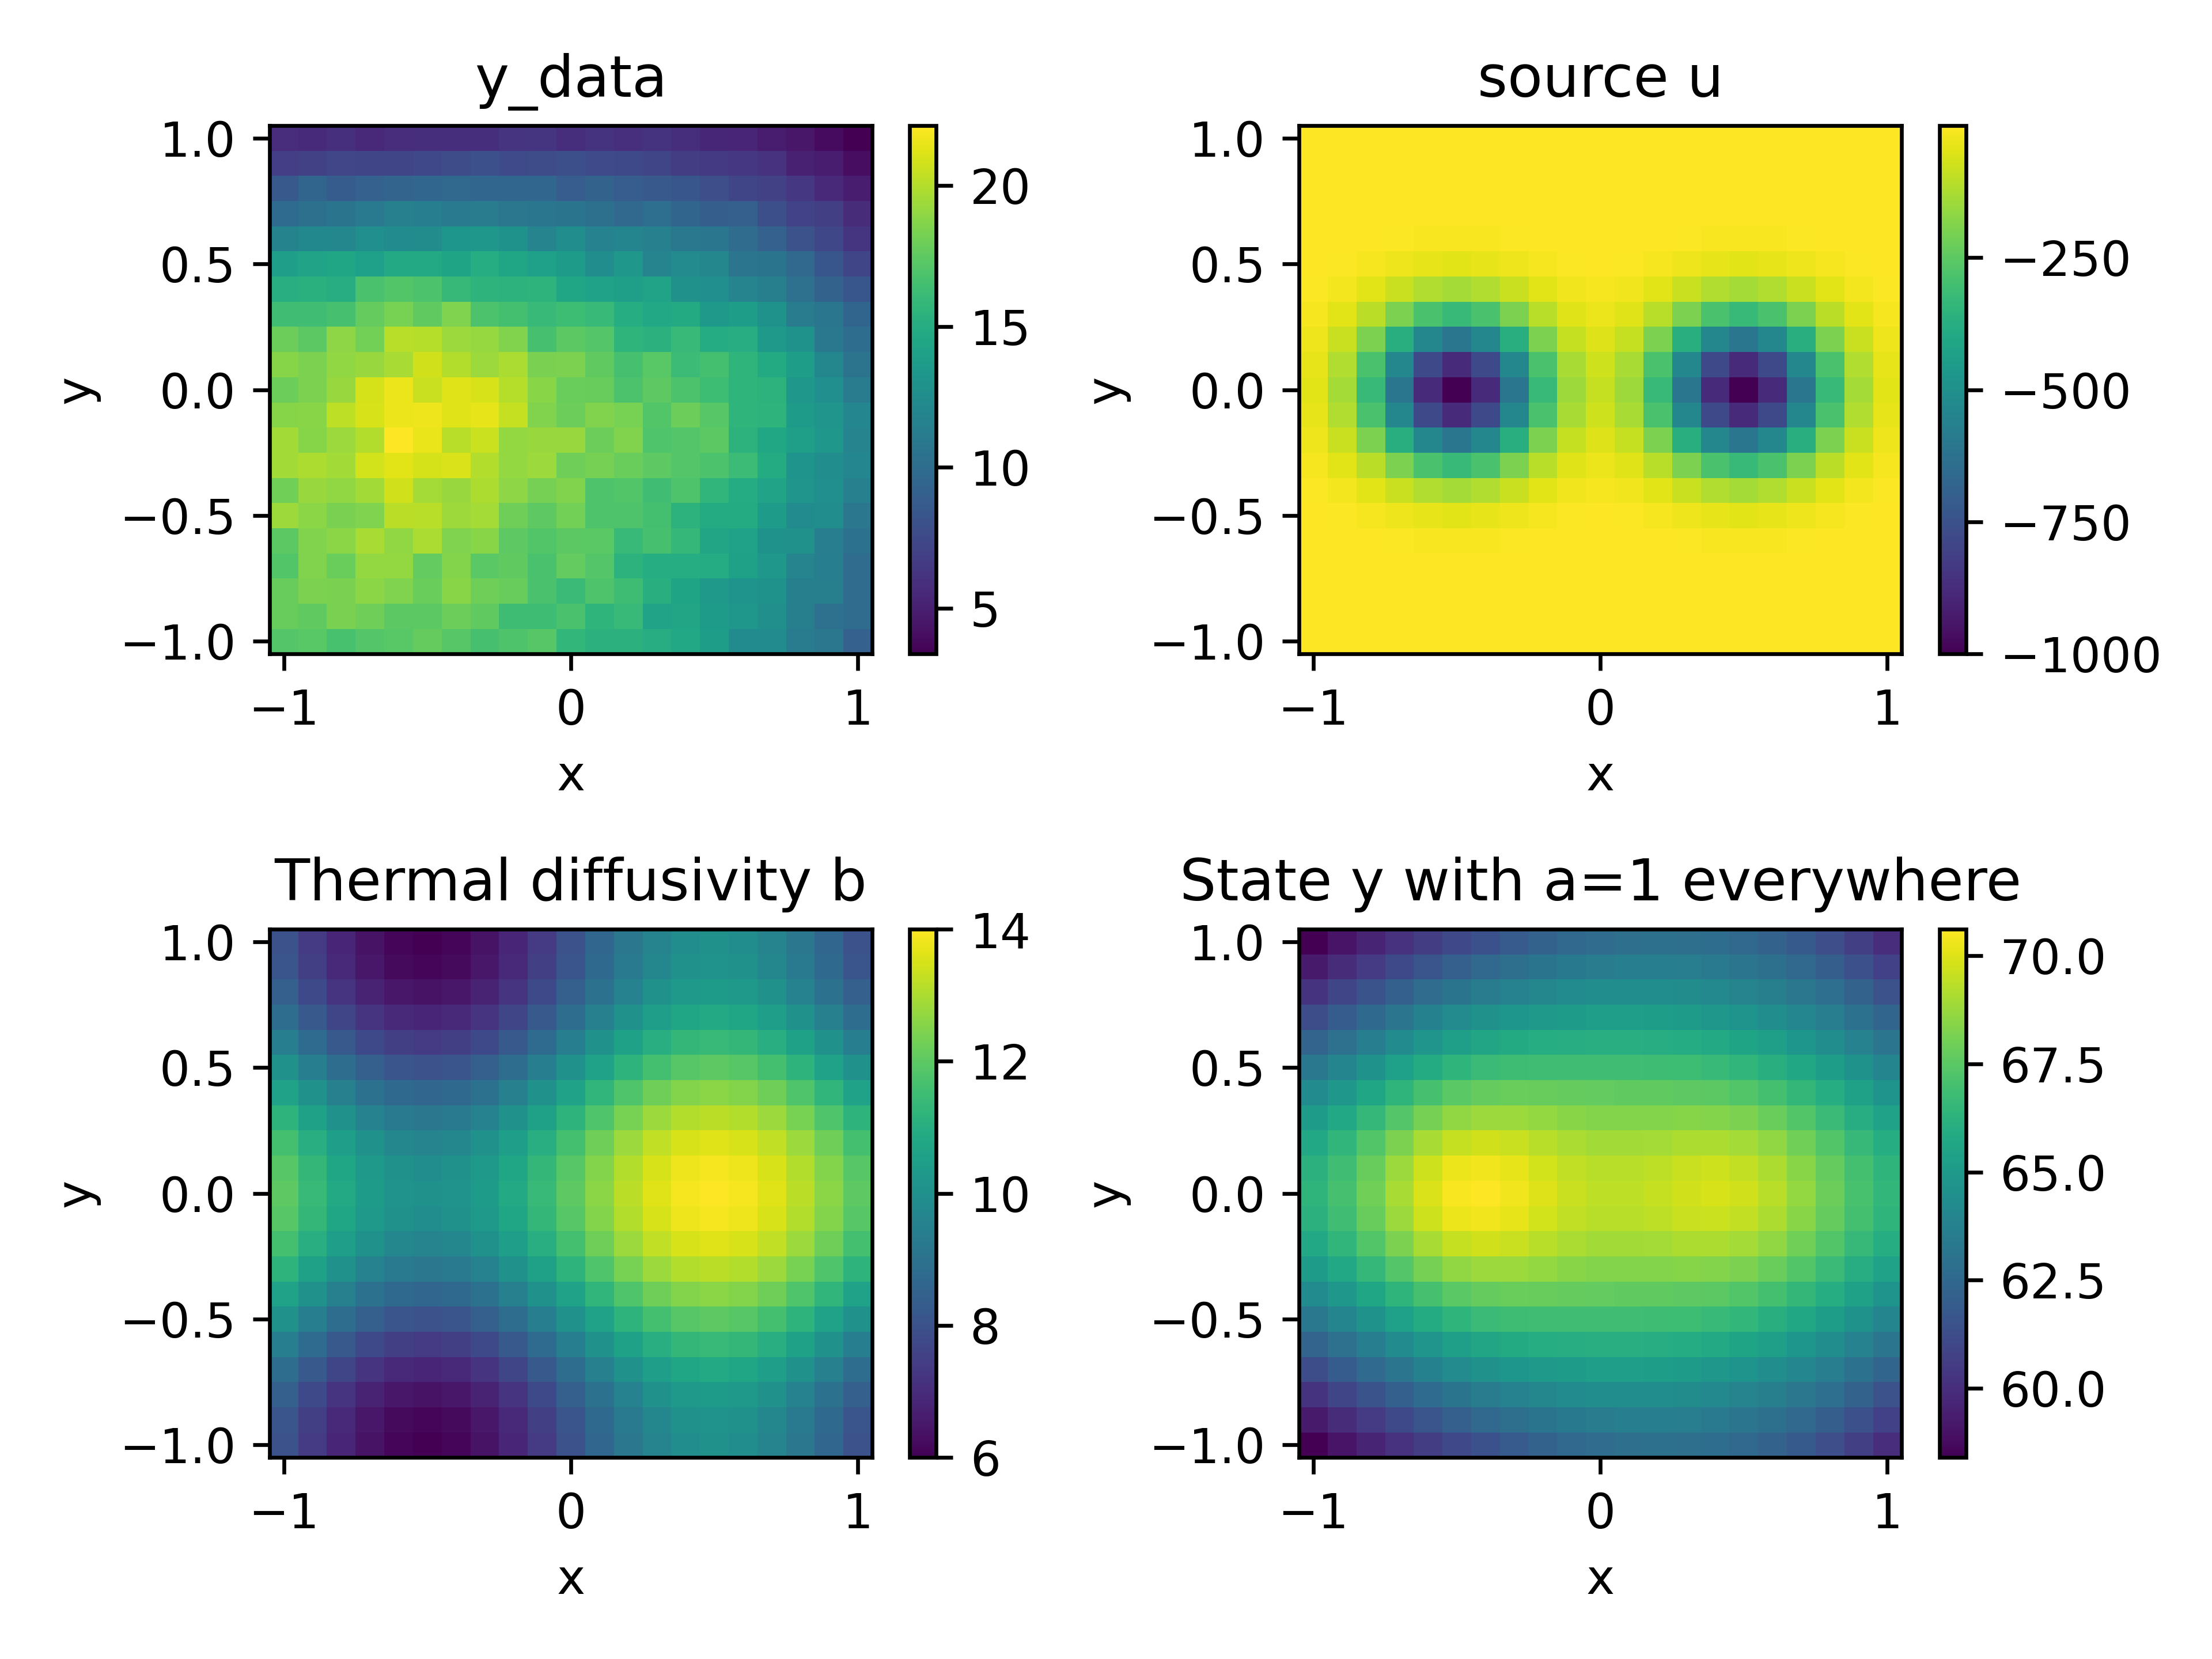
\includegraphics[width=0.8\linewidth]{Project/Part1/Figures/setup.png}
    \caption{Problem setup.}
    \label{fig:p1_setup}
\end{figure}




\paragraph{Prior knowledge}
\begin{itemize}
  \item Initial guess $a_0(\bx)=1$.
  \item $a(\bx)>0$: This can be exploited through reparametrization. 
  \item $a(\bx)$ is piecewise constant along $\dOm$ and may have discontinuities: Motivates TV regularization, which promotes piecewise smooth solutions with discontinuities. 
 \item $y_d$ is noisy with uniform errors $\pm10\%$: Motivates regularization for less overfitting. 
\end{itemize}



\section{Theory}
\subsection{Cost functional} 
I define the cost functional as: 
\begin{equation}
\boxed{\;
\mathcal{J}(y)=\frac12\int_\Om (y-\yd)^2\dd\bx \;}
\end{equation}


\subsection{Lagrangian}
In order to optimize the cost, we need to find the gradient with respect to $a$. This can be done via the adjoint method. Form the Lagrangian:
\begin{equation}
\mathcal{L}(y,\yadj,a)=\mathcal{J}(y)+\int_\Om \yadj\,\big(\nabla\cdot b\nabla y-u\big)\dd\bx .
\end{equation}
Applying Green's identity twice to the first term in the Lagrangian, and using the boundary condition
$b\,\pn y=-a y$,
\begin{align*}
\int_\Om \yadj\,\nabla\cdot b\nabla y\dd\bx
&=\int_{\dOm}\yadj\, b\,\pn y\dd s-\int_\Om\nabla\yadj\cdot b\nabla y\dd\bx \nonumber\\
&=-\int_{\dOm}a\,\yadj y\dd s-\int_{\dOm}y\,b\,\pn\yadj\dd s+\int_\Om y\,\nabla\cdot b\nabla\yadj\dd\bx \nonumber\\
&=\int_\Om y\,\nabla\cdot b\nabla\yadj\dd\bx-\int_{\dOm}y\big(b\,\pn\yadj+a\,\yadj\big)\dd s .
\end{align*}
Therefore
\begin{equation}
\boxed{\;
\mathcal{L}(y,\yadj,a)=\mathcal{J}(y)+\int_\Om\big(y\,\nabla\cdot b\nabla\yadj-\yadj u\big)\dd\bx
-\int_{\dOm}y\big(b\,\pn\yadj+a\,\yadj\big)\dd s\;}
\end{equation}


\subsection{Continuous adjoint gradient}
%==========================================================
\paragraph{Variation with respect to $\mathbf{y}$:}
\begin{align*}
\delta_y\mathcal{L}
&=\underbrace{\int_\Om (y-\yd)\,\delta y\dd\bx}_{\delta_y\mathcal{J}}
+\int_\Om\delta y\,\nabla\cdot b\nabla\yadj\dd\bx
-\int_{\dOm}\delta y\big(b\,\pn\yadj+a\,\yadj\big)\dd s \nonumber\\
&=\int_\Om\big(\nabla\cdot b\nabla\yadj+y-\yd\big)\delta y\dd\bx
-\int_{\dOm}\big(b\,\pn\yadj+a\,\yadj\big)\delta y\dd s\overset{!}{=}0 .
\end{align*}
Requiring this to vanish for all $\delta y$ gives the adjoint PDE and adjoint BC \eqref{eq:adjoint_cont}:
\begin{equation}
\boxed{\;
\begin{cases}
\nabla\cdot b\nabla\yadj=\yd-y, & \bx\in\Om,\\
b\,\pn\yadj+a\,\yadj=0, & \bx\in\dOm.
\end{cases}}
\label{eq:adjoint_cont}
\end{equation}
This is the same as the heat equation, but with a new source term $\yd-y$.

\paragraph{Variation with respect to $\mathbf{a}$:}
\begin{equation}
\delta_a\mathcal{L}=\int_{\dOm}\big(-y\,\yadj\big)\,\delta a\dd s .
\end{equation}
If the PDE is satisfied then $\mathcal{J}=\mathcal{L}$, so
\begin{equation}
\boxed{\;\frac{\delta\mathcal{J}}{\delta a}=\frac{\delta\mathcal{L}}{\delta a}=-\,y\,\yadj\Big|_{\dOm}\;}
\end{equation}


\subsection{Discrete adjoint gradient}
\subsubsection{Discretization}
Let $y,\yd,u\in\mathbb{R}^{m_x \times m_y}$ be grid functions and $H$ the SBP quadrature matrix.
The discrete cost is then
\begin{equation}
J(y)=\frac12 (y-\yd)^T H\,(y-\yd).
\end{equation}
The SBT-SAT discretization of equation \eqref{eq:pde} is
\begin{equation}
(D_{x_1}^{+}BD_{x_1}^{-}+D_{x_2}^{+}BD_{x_2}^{-})y
=u+H^{-1}\eb\,\Hb\big(\Bb\, d_n^{T}y+A\,\eb^{T}y\big),
\end{equation}
which can be written compactly as
\begin{equation}
\boxed{D(a)\,y=u},\qquad
D=D_{x_1}^{+}BD_{x_1}^{-}+D_{x_2}^{+}BD_{x_2}^{-}-H^{-1}\eb\,\Hb\big(\Bb\, d_n^{T}+A\,\eb^{T}\big).
\end{equation}
Here
\begin{equation}
B=\operatorname{diag}(b),\qquad
\Bb=\begin{bmatrix}
e_W^TBe_W & & &\\
& e_S^TBe_S & &\\
& & e_E^TBe_E &\\
& & & e_N^TBe_N
\end{bmatrix},\qquad
A=\operatorname{diag}(a)
\end{equation}
where $a\in\mathbb{R}^{n_{\partial\Omega}}$ holds the values of $a$ at the boundary
grid points (ordered $W,S,E,N$ as in $\eb$), and $A$ is its diagonal matrix.

\subsubsection{Discrete adjoint method}
%==========================================================
The discrete Lagrangian is
\begin{equation}
L(y,\yadj,a)=J(y)+(\yadj)^TH\big(D(a)\,y-u\big).
\end{equation}

\paragraph{Discrete adjoint equation:}
Differentiating with respect to $y$ and using
$HD=D^TH$,
\begin{align*}
\frac{\partial L}{\partial y}
= & (y-\yd)^TH+(\yadj)^TH D(a)
=(y-\yd)^TH+(\yadj)^TD(a)^TH \\
= & \big(y-\yd+D(a)\,\yadj\big)^TH \overset{!}{=}0
\end{align*}
which gives the discrete adjoint PDE \eqref{eq:adjoint_disc}:
\begin{equation}
\boxed{D(a)\,\yadj=\yd-y.}
\label{eq:adjoint_disc}
\end{equation}

\paragraph{Discrete gradient with respect to $\mathbf{a}:$}
The SBP property gives
\begin{align*}
(\yadj)^TH D\,y
&=-(D_{x_1}^{-}\yadj)^TH B D_{x_1}^{-}y-(D_{x_2}^{-}\yadj)^TH B D_{x_2}^{-}y \nonumber\\
&\quad+(\eb^T\yadj)^T\Hb\big(\eb^T\Bb\,d_n^Ty\big)-(\eb^T\yadj)^T\Hb\big(\eb^T\Bb\,d_n^Ty\big)-(\yadj)^T\eb\Hb A\,\eb^Ty \\
&=-(D_{x_1}^{-}\yadj)^THBD_{x_1}^{-}y-(D_{x_2}^{-}\yadj)^THBD_{x_2}^{-}y
-(\eb^T\yadj)^T\Hb\,A\,(\eb^Ty)
\end{align*}

Rewriting $L$ with this identity,
\begin{equation*}
L(y,\yadj,a)=J(y)-(D_{x_1}^{-}\yadj)^THBD_{x_1}^{-}y-(D_{x_2}^{-}\yadj)^THBD_{x_2}^{-}y
-(\eb^T\yadj)^T\Hb\,A\,(\eb^Ty)-(\yadj)^THu .
\end{equation*}
Only the boundary term depends on $a$. Using $\dfrac{\partial}{\partial a}\big(v^TAw\big)=v\odot w$,
\begin{equation}
\boxed{\;\frac{\partial L}{\partial a}=-\Hb\,\big(\eb^T\yadj\big)\odot\big(\eb^Ty\big)\;}
\end{equation}
This matches the continuous gradient $-y\,\yadj|_{\dOm}$, with the quadrature weights $\Hb$
coming from the discrete boundary integral.

%==========================================================
\subsection{Reparametrization}
%==========================================================
Since $a(\bx)>0$, enforce positivity by writing
\begin{equation}
a=a_0+a_\ell^{2}
\quad\Longleftrightarrow\quad
a_\ell=\sqrt{a-a_0},\qquad a_0=10^{-6}.
\label{eq:p1_reparametrization}
\end{equation}
By the chain rule,
\begin{equation}
\nabla_{a_\ell}J=\nabla_aJ \, \frac{\partial a}{\partial a_\ell}=2\,\nabla_aJ\odot a_\ell
\end{equation}

%==========================================================
\subsection{TV regularization}
%==========================================================
Since $a(\bx)$ is expected to be piecewise smooth along $\dOm$, we add a total
variation penalty with strength $\varepsilon>0$:
\begin{equation}
\mathcal{J}(y)\;\longrightarrow\;\mathcal{J}(y)+\varepsilon\mathcal{R}(a).
\end{equation}
The gradient then becomes:
\begin{equation}
\nabla_a\mathcal{J}(y)\;\longrightarrow\;\nabla_a\mathcal{J}(y)+\varepsilon\nabla_a\mathcal{R}(a),
\end{equation}
\subsubsection{Continuous case}
The TV functional is
\begin{equation}
\mathcal{R}(a)=\Big\|\frac{\partial a}{\partial s}\Big\|_{L^1(\dOm)}=\int_{\dOm}\Big|\frac{\partial a}{\partial s}\Big|\dd s
\end{equation}
It is not differentiable where $\partial_s a=0$, so we use the smoothed version
\begin{equation}
\mathcal{R}(a)=\int_{\dOm}\sqrt{(\partial_s a)^2+\gamma^2}\dd s,\qquad \gamma>0,\;\text{ choose }\gamma=10^{-6}.
\end{equation}

\paragraph{First variation with respect to $\mathbf{a}$:}
\begin{equation}
\delta_a\mathcal{R}=\int_{\dOm}\frac{\partial_s a}{\sqrt{(\partial_s a)^2+\gamma^2}}\,\delta(\partial_s a)\dd s
=-\int_{\dOm}\partial_s\!\left(\frac{\partial_s a}{\sqrt{(\partial_s a)^2+\gamma^2}}\right)\delta a\dd s ,
\end{equation}
where integration by parts on the closed curve $\dOm$ produces no boundary terms. Hence
\begin{equation}
\boxed{\;\frac{\delta\mathcal{R}}{\delta a}=-\frac{\partial}{\partial s}\!\left(\frac{\partial_s a}{\sqrt{(\partial_s a)^2+\gamma^2}}\right)
\;}
\end{equation}

\subsubsection{Discrete case}
Let $D_t$ be the tangential derivative operator along $\dOm$,
$\Hb$ the boundary quadrature, and $\one$ a vector of ones. Squares, square roots and powers of
vectors are taken elementwise. Define
\begin{equation}
R(a)=\one^T\Hb\sqrt{(D_ta)^2+\gamma^2}=\one^T\Hb\sqrt{W(a)},\quad \gamma=10^{-6}.
\end{equation}
By the chain rule,
\begin{equation}
\nabla_aR(a)=\tfrac12\,\one^T\Hb\operatorname{diag}\!\big(W(a)^{-1/2}\big)\,\nabla_aW(a),
\qquad
\nabla_aW(a)=\operatorname{diag}(2D_ta)\,D_t ,
\end{equation}
so that
\begin{equation}
\boxed{\;\nabla_aR(a)=\one^T\Hb\operatorname{diag}\!\big(W(a)^{-1/2}\big)\operatorname{diag}(D_ta)\,D_t\;}
\end{equation}



\section{Results}
\subsection{Adjoint gradient}
The adjoint gradient $\frac{\partial L}{\partial a}$ compared to the finite difference (FD) gradient can be seen in Figure~\ref{fig:p1_gradient_comparison}. The difference is small, and therefore the adjoint gradient can be assumed to be correctly implemented. 

\begin{figure}[H]
    \centering
     \begin{subfigure}[b]{0.45\textwidth}
        \centering
        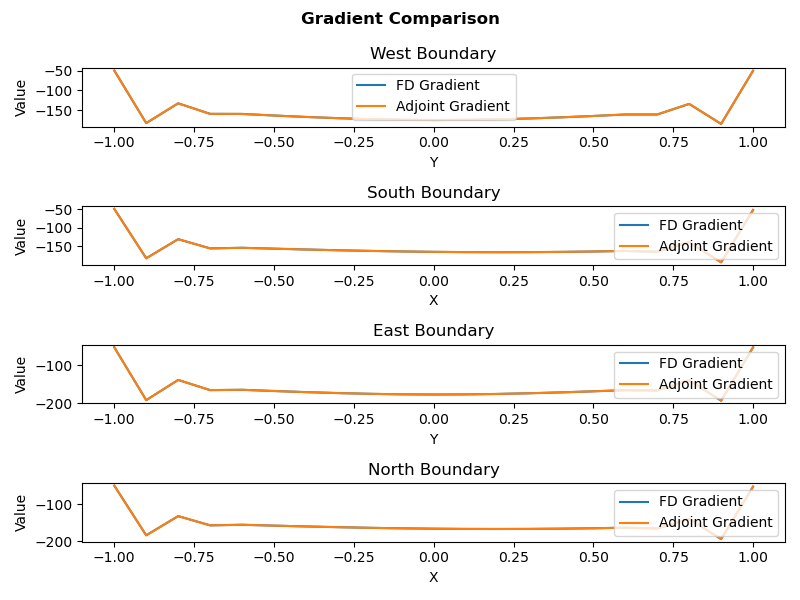
\includegraphics[width=\textwidth]{Project/Part1/Figures/gradient_comparison.png}
        \caption{Gradient $\frac{\partial L}{\partial a}$.}
    \end{subfigure}
    \hfill
    \begin{subfigure}[b]{0.45\textwidth}
        \centering
        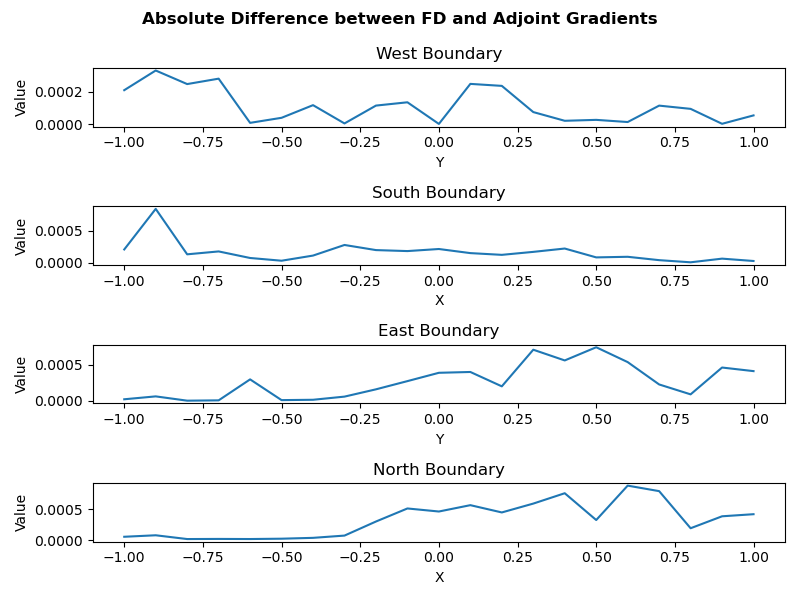
\includegraphics[width=\textwidth]{Project/Part1/Figures/gradient_difference.png}
        \caption{Absolute difference.}
    \end{subfigure}
    \caption{Comparison between different gradient calculation methods.}
    \label{fig:p1_gradient_comparison}
\end{figure}

\subsection{First optimization}
Without regularizing or reparameterization, the optimized $a$ was reached after $482$ BFGS iterations and at a final data mismatch cost $J \approx 1.307$ (Figure~\ref{fig:p1_initial_optimization}). 

\begin{figure}[H]
    \centering
     \begin{subfigure}[b]{0.55\textwidth}
        \centering
        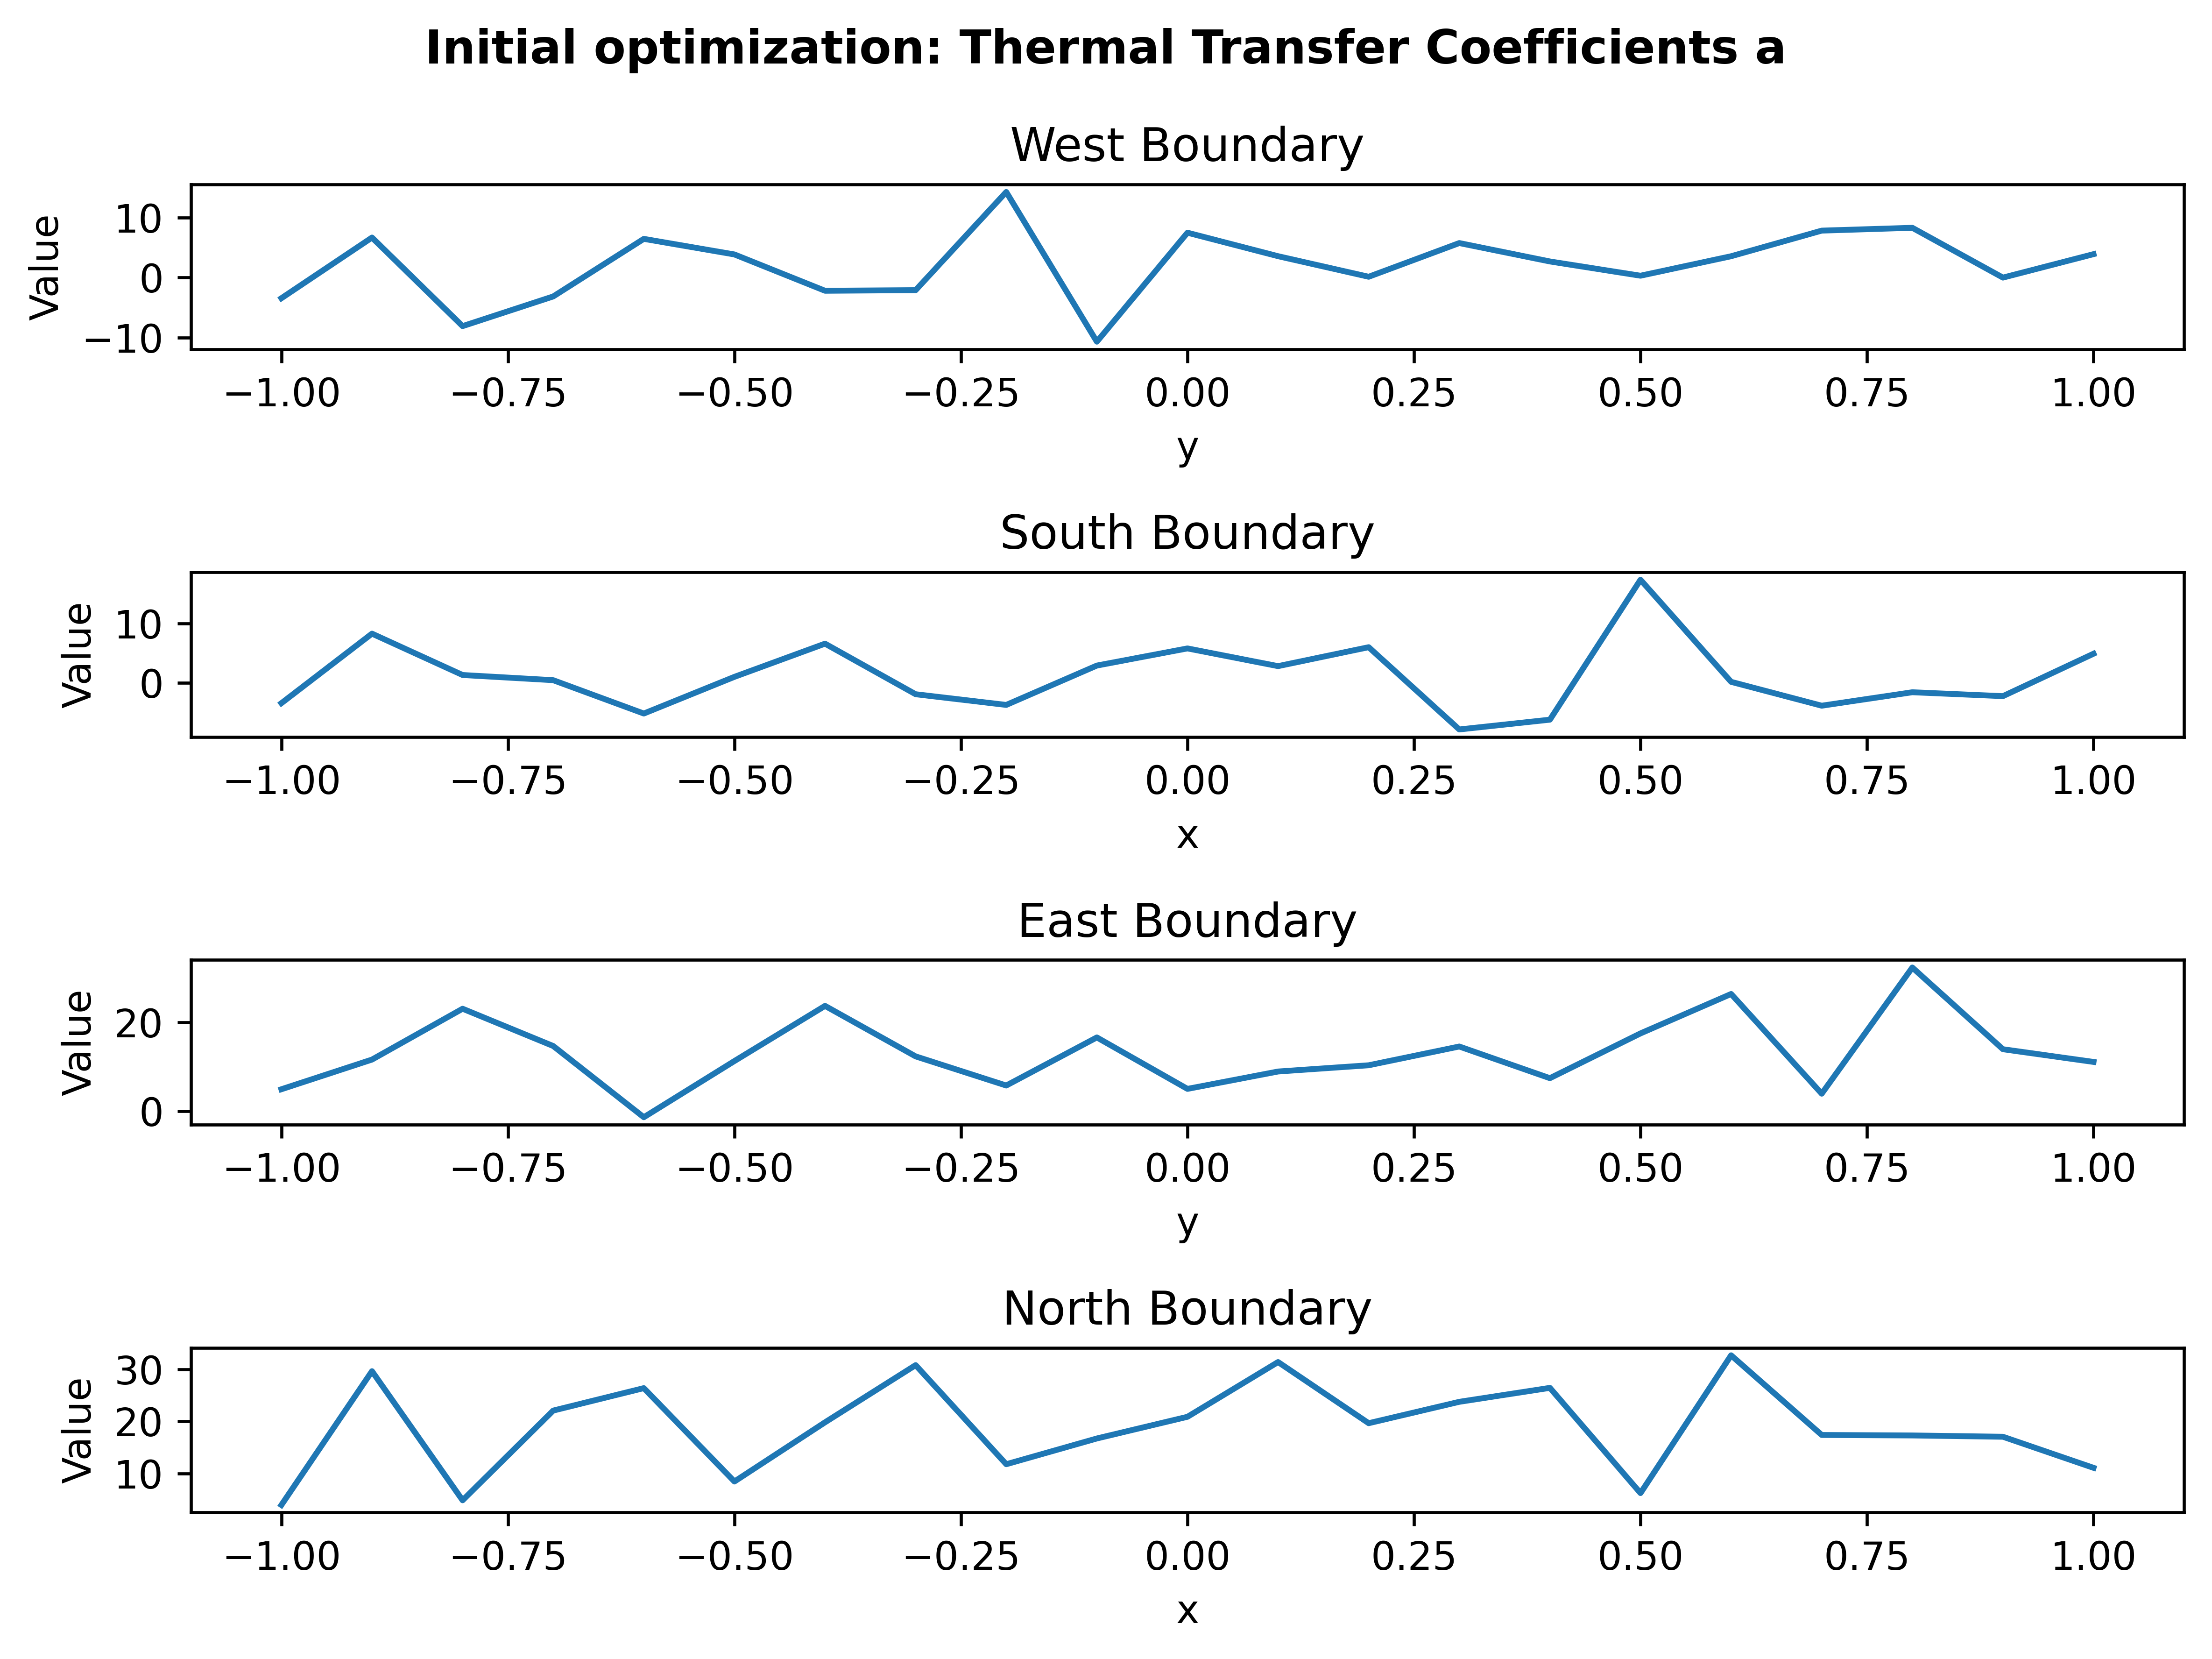
\includegraphics[width=\textwidth]{Project/Part1/Figures/initial_optimization_a.png}
        \caption{Optimized $a$ solution.}
    \end{subfigure}
    \hfill
    \begin{subfigure}[b]{0.40\textwidth}
        \centering
        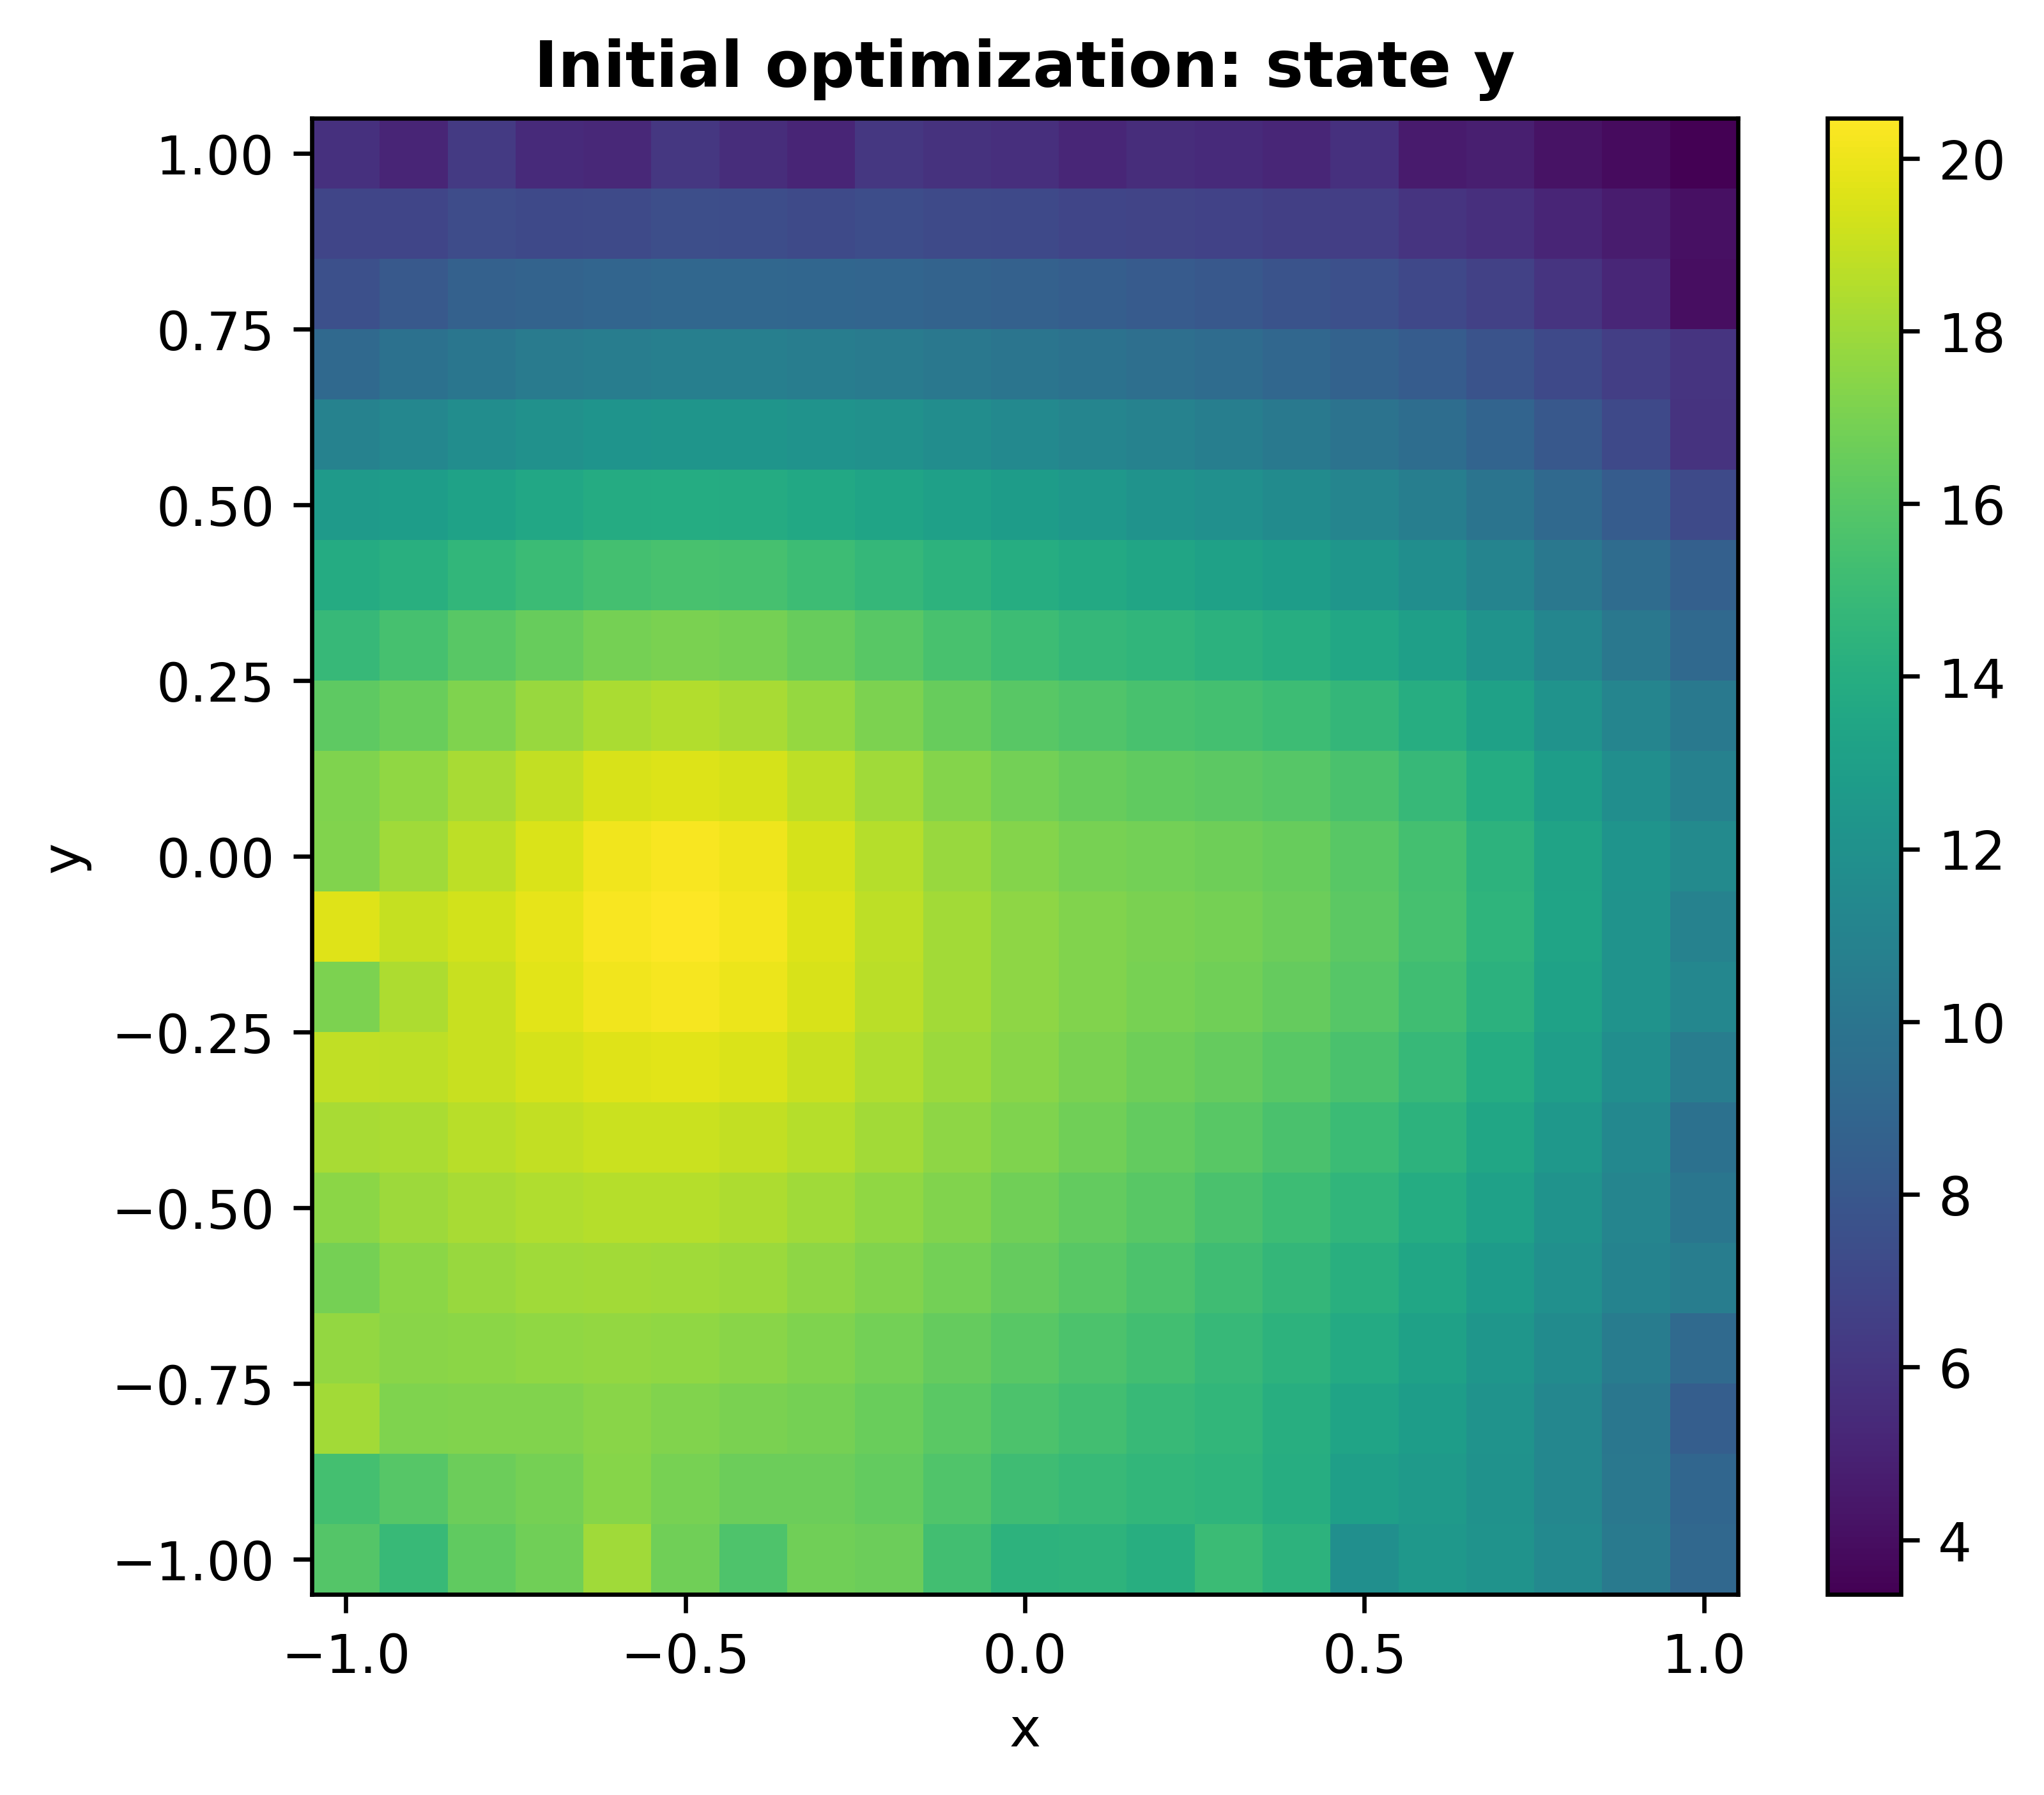
\includegraphics[width=\textwidth]{Project/Part1/Figures/initial_optimization_y.png}
        \caption{Optimized state $y$.}
    \end{subfigure}
    \caption{Initial solution of inversion problem. }
    \label{fig:p1_initial_optimization}
\end{figure}

\subsection{Reparameterization}
By utilising the reparametrization \eqref{eq:p1_reparametrization}, an optimized $a$ was reached after $622$ BFGS iterations and at a final data mismatch cost $J \approx 1.332$ (Figure~\ref{fig:p1_reparam_optimization}). 


\begin{figure}[H]
    \centering
     \begin{subfigure}[b]{0.55\textwidth}
        \centering
        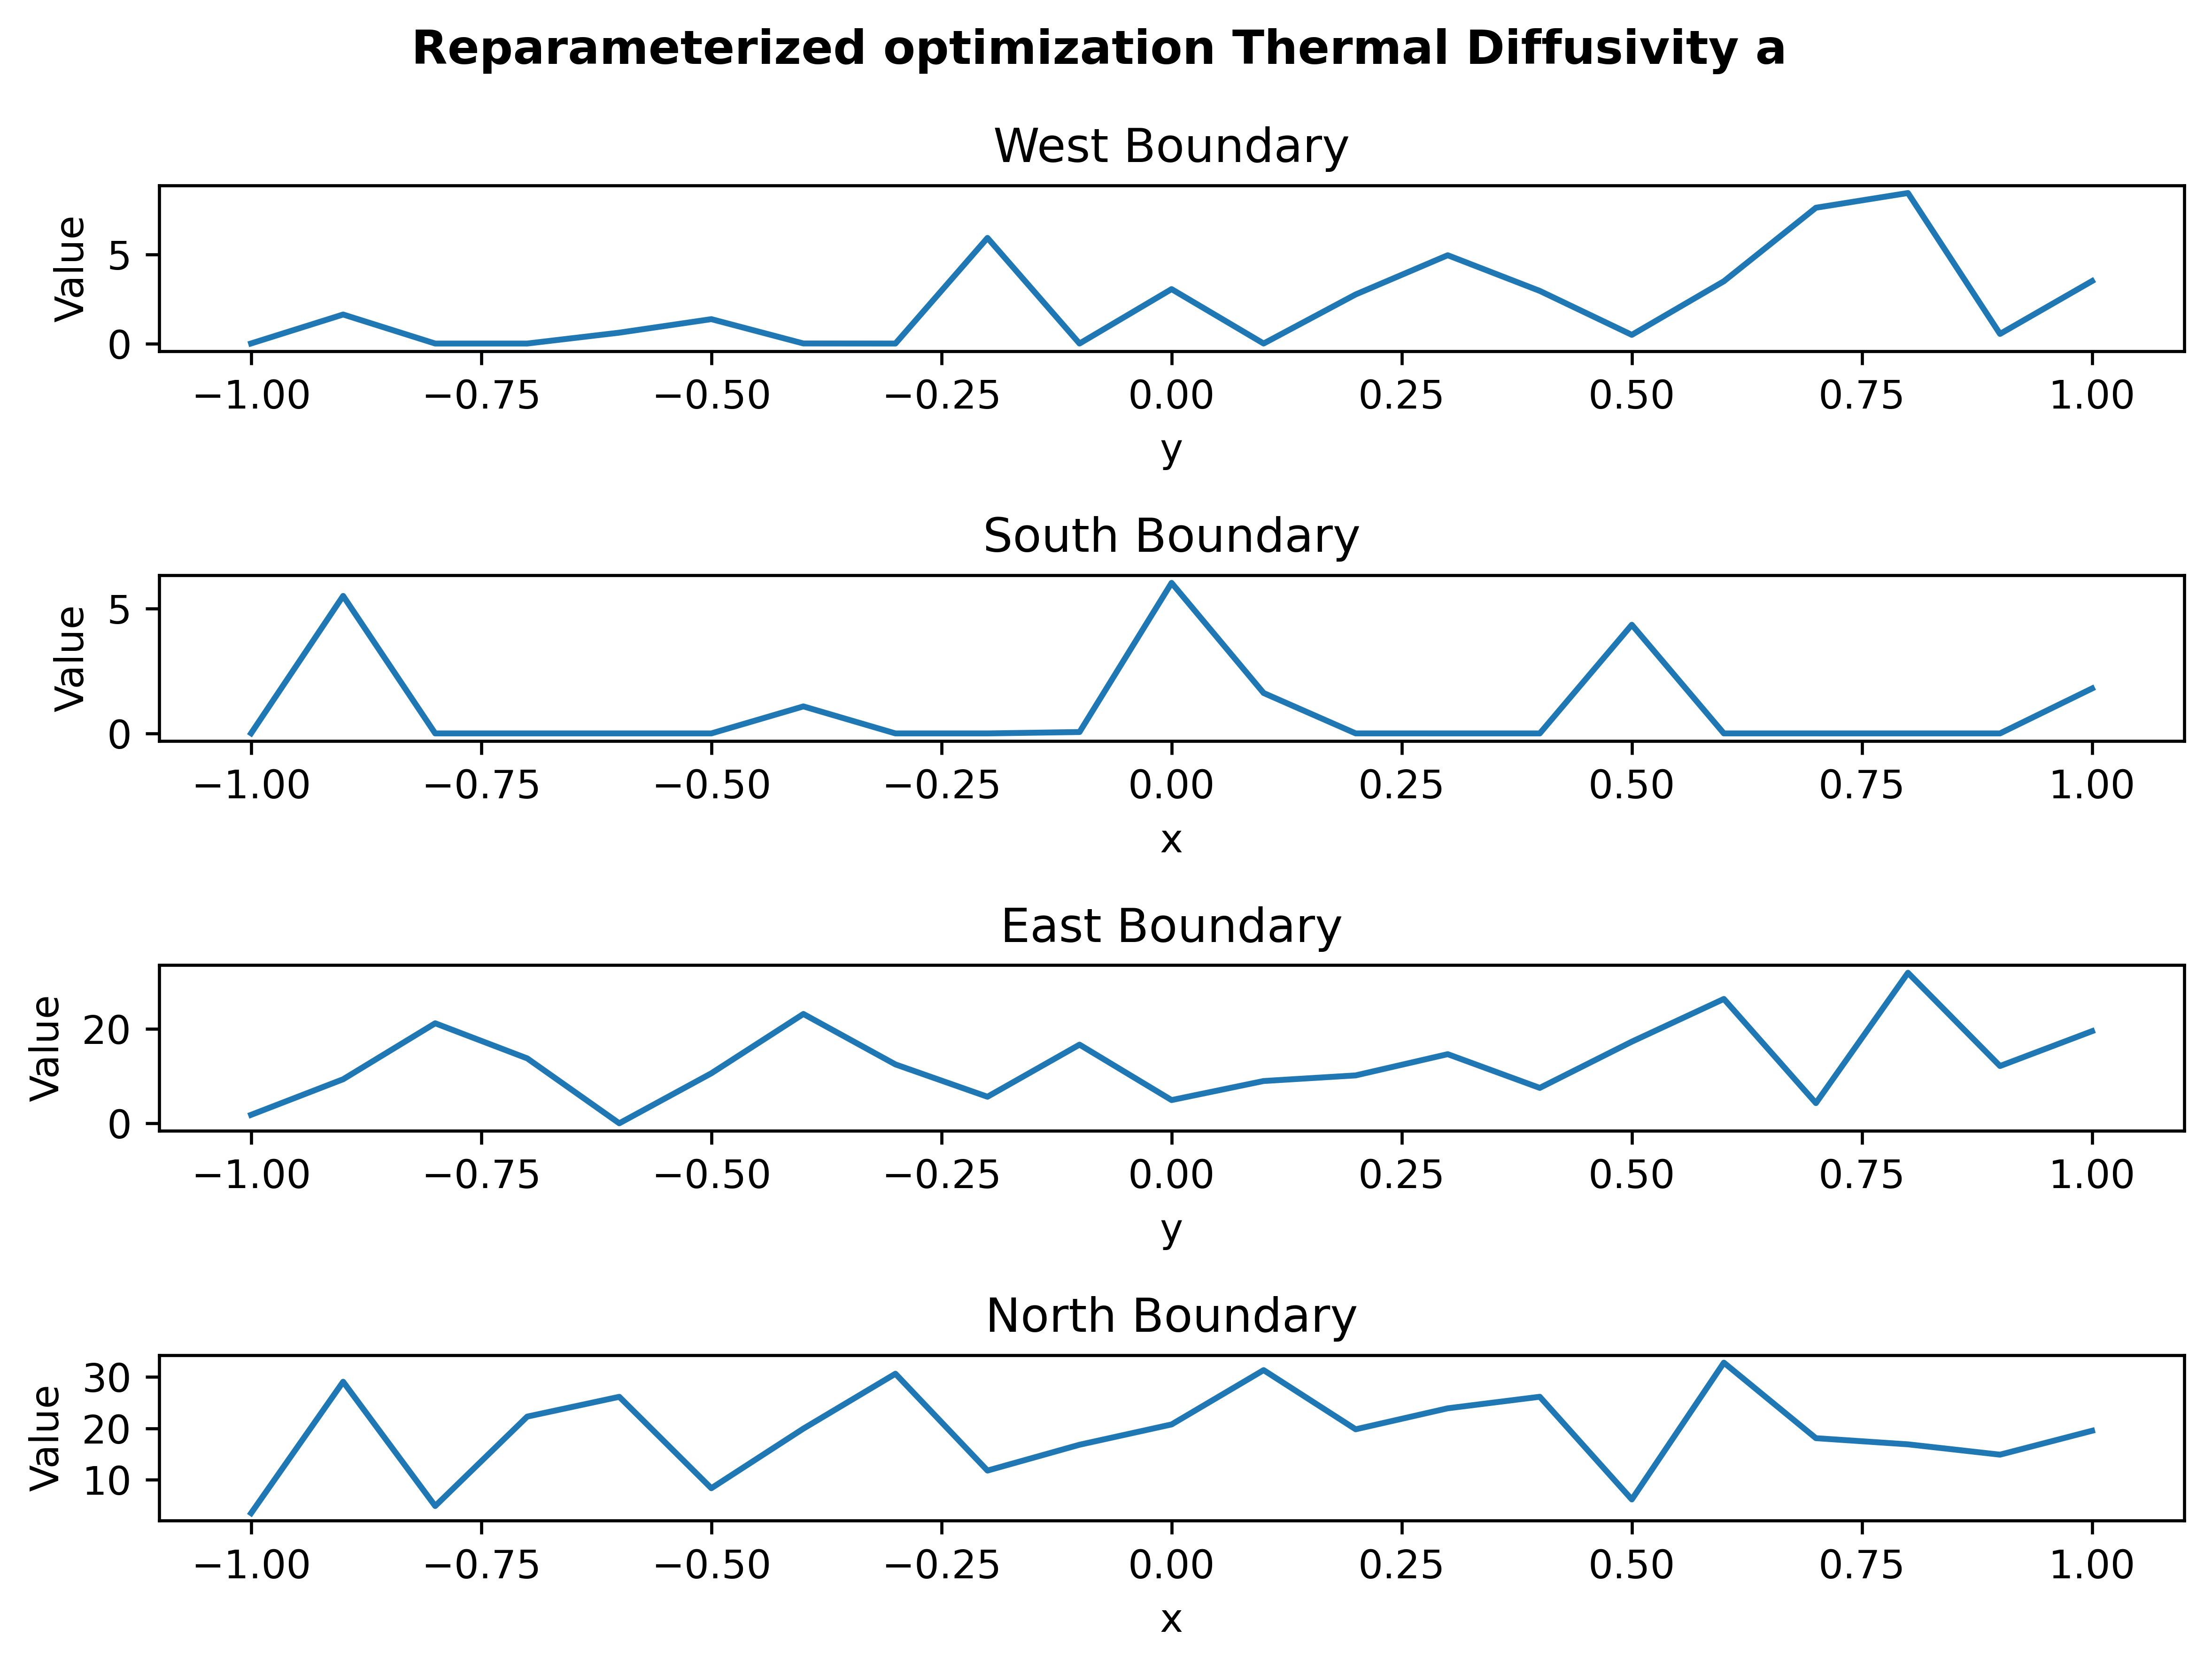
\includegraphics[width=\textwidth]{Project/Part1/Figures/reparam_optimization_a.png}
        \caption{Optimized $a$ solution.}
    \end{subfigure}
    \hfill
    \begin{subfigure}[b]{0.40\textwidth}
        \centering
        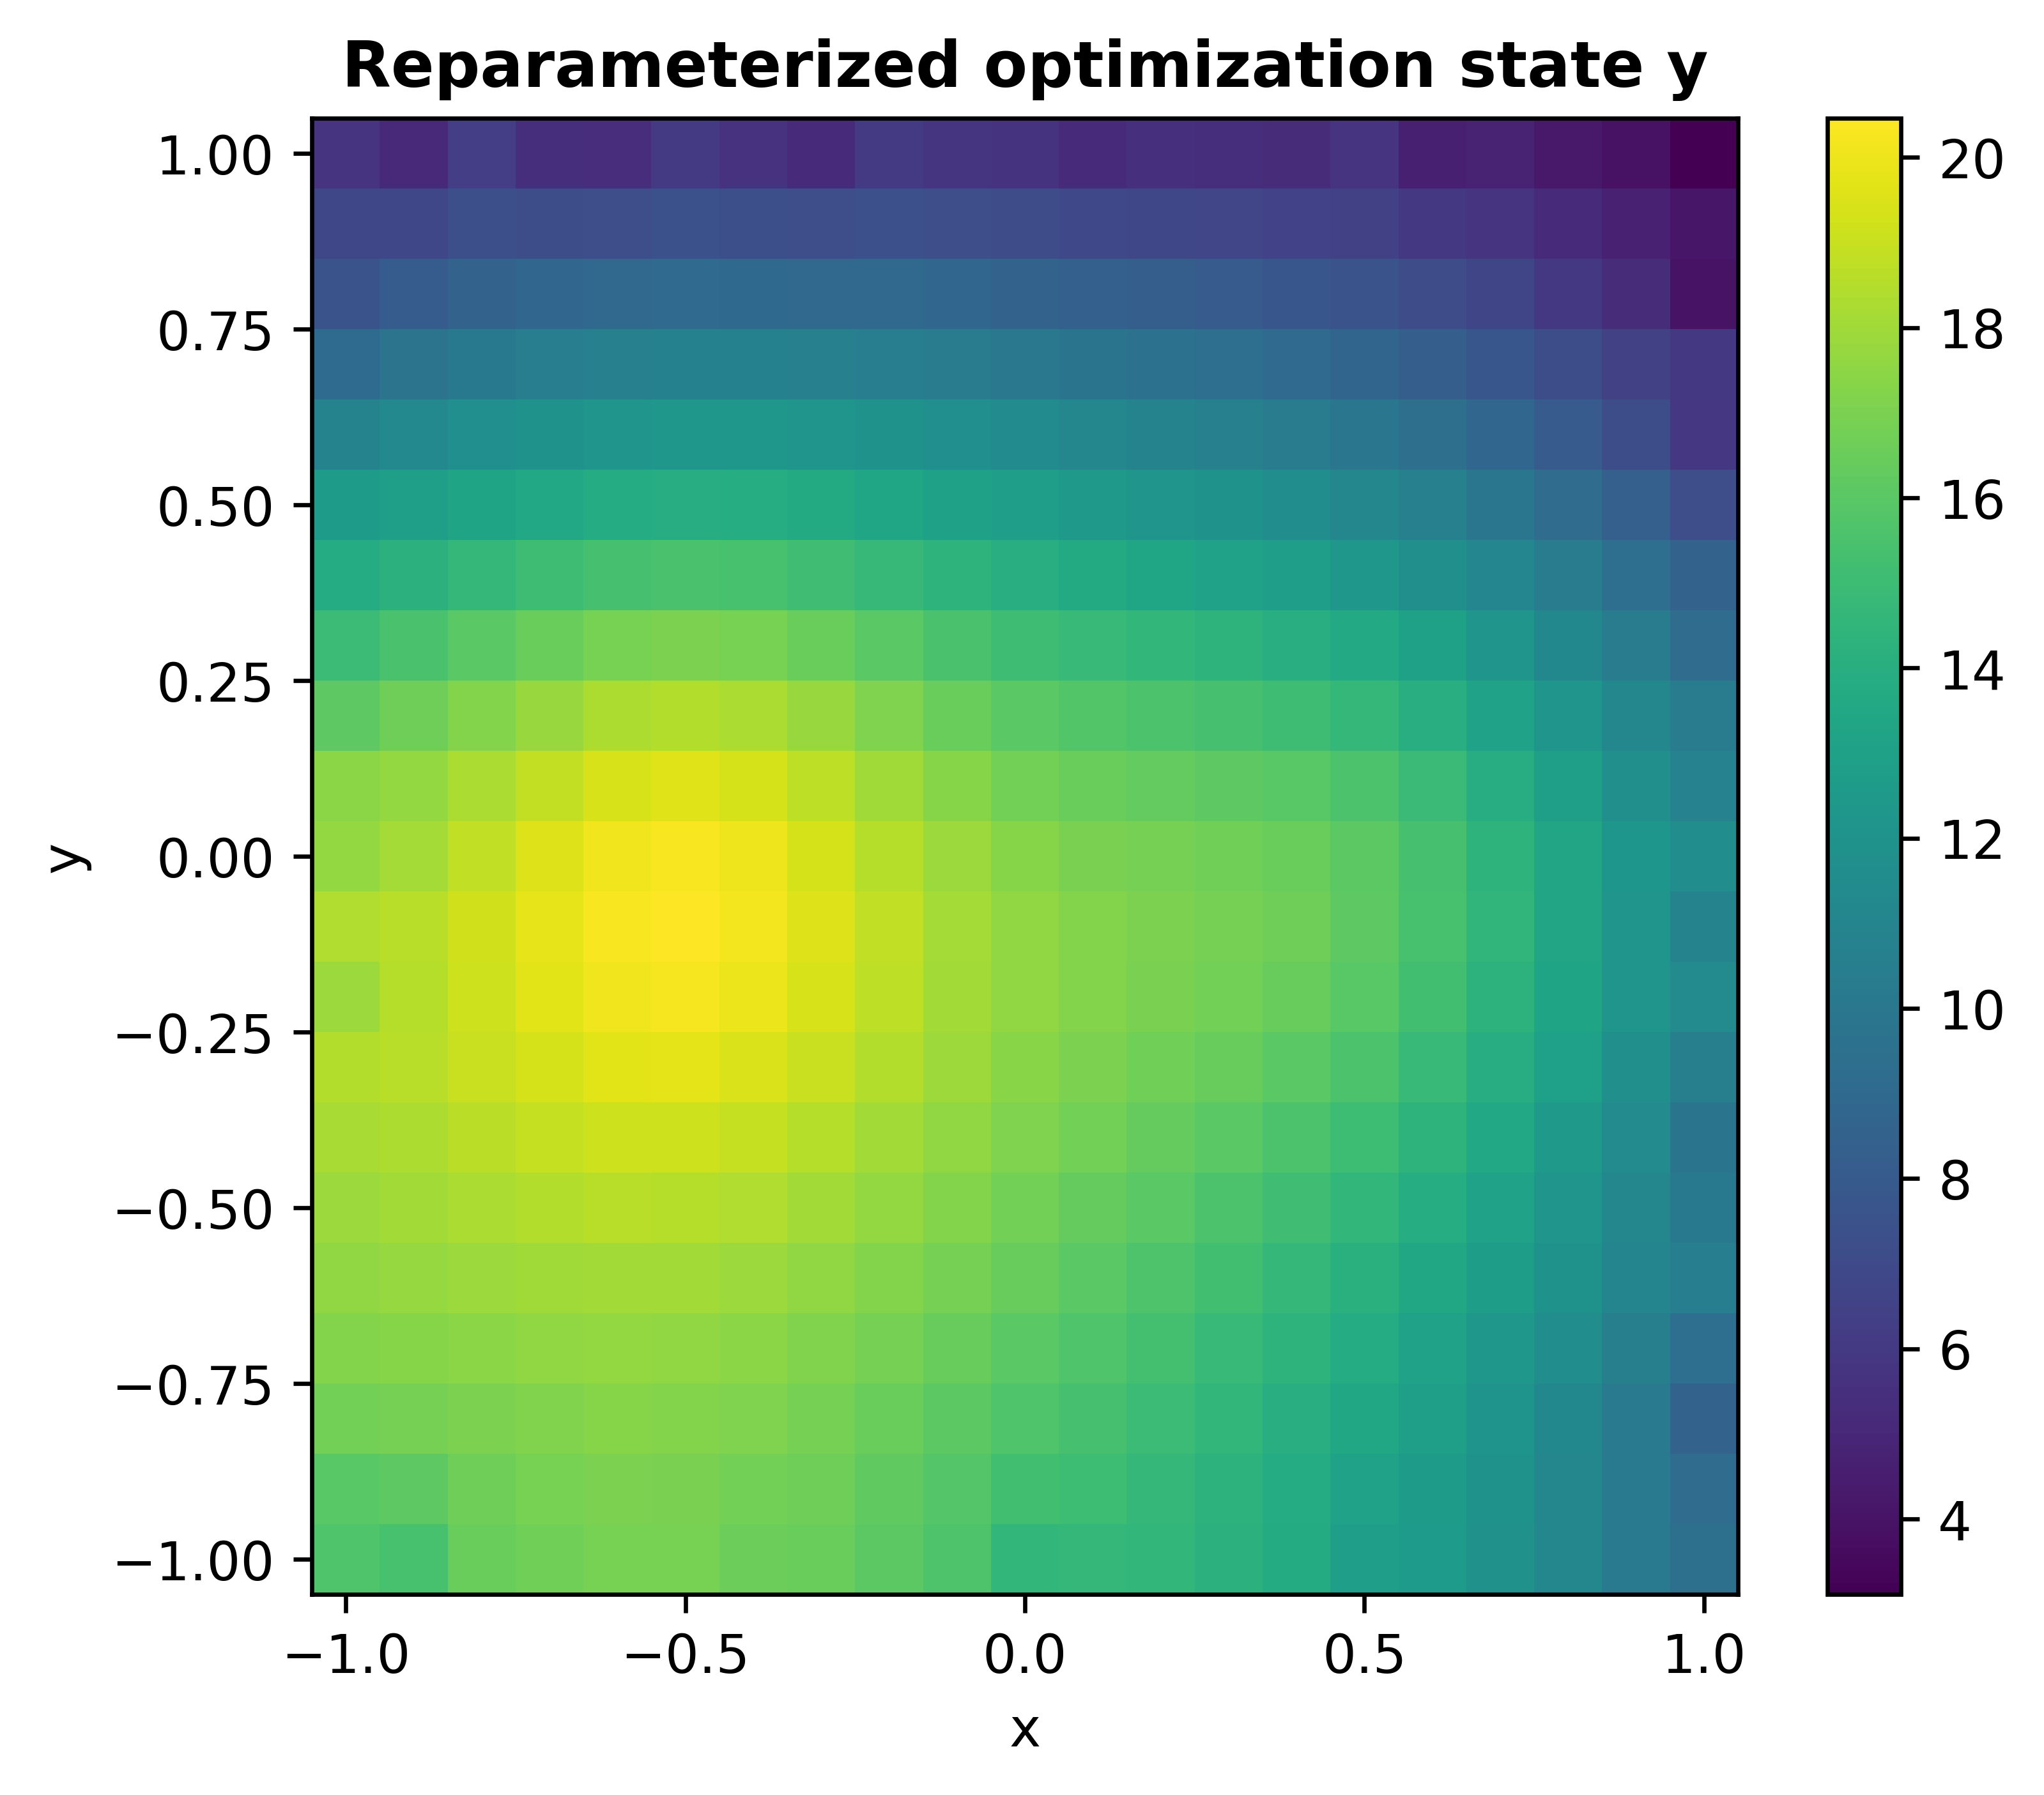
\includegraphics[width=\textwidth]{Project/Part1/Figures/reparam_optimization_y.png}
        \caption{Optimized state $y$.}
    \end{subfigure}
    \caption{Reparameterized solution of inversion problem. }
    \label{fig:p1_reparam_optimization}
\end{figure}

\subsection{Regularized and reparameterized optimization}
Using both reparameterization and TV--regularization, the final $a$ solution can be found. First, the TV--gradient must be validated (Figure~\ref{fig:p1_TV_gradient_comparison}) and the optimal $\varepsilon$ value be found (Figure~\ref{fig:p1_epsilon_error_norm}).

\begin{figure}[H]
    \centering
     \begin{subfigure}[b]{0.45\textwidth}
        \centering
        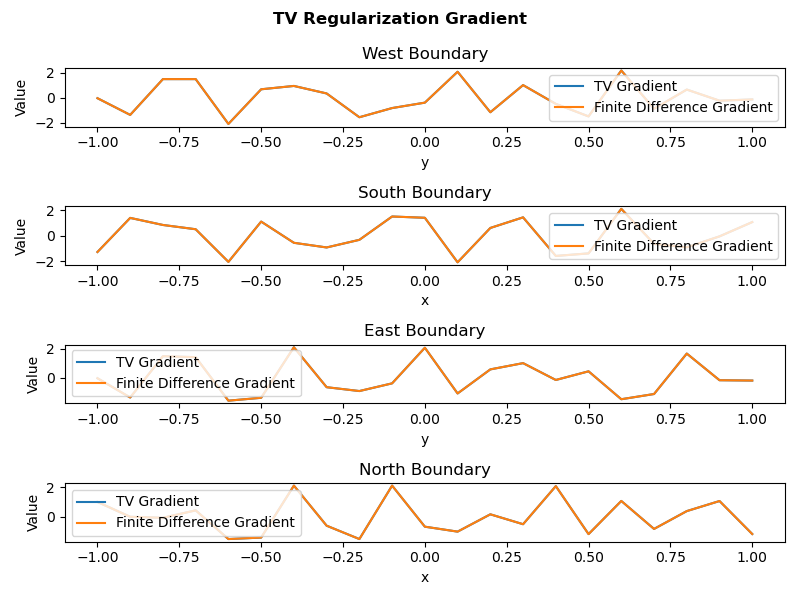
\includegraphics[width=\textwidth]{Project/Part1/Figures/TV_gradient_comparison.png}
        \caption{Gradient $\nabla_aR(a)$.}
    \end{subfigure}
    \hfill
    \begin{subfigure}[b]{0.45\textwidth}
        \centering
        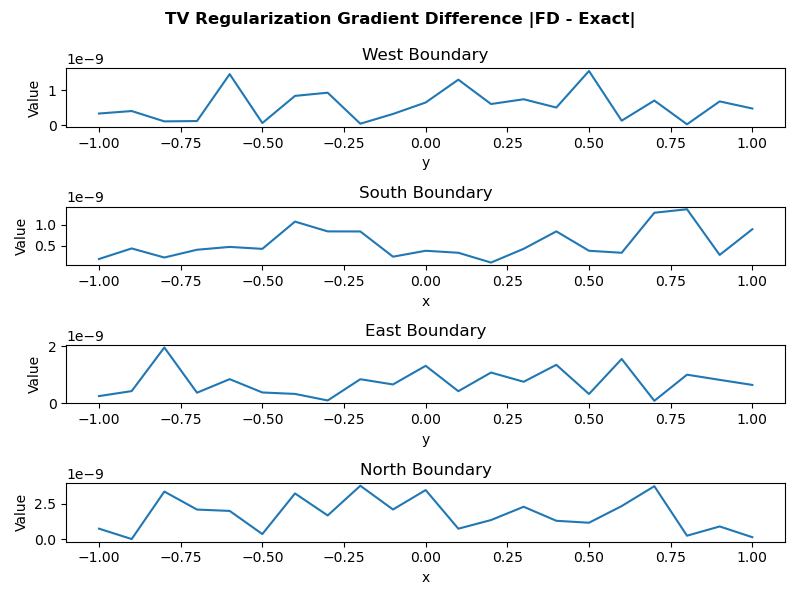
\includegraphics[width=\textwidth]{Project/Part1/Figures/TV_gradient_difference.png}
        \caption{Absolute difference.}
    \end{subfigure}
    \caption{Comparison between different gradient calculation methods for the TV--regularization gradient.}
    \label{fig:p1_TV_gradient_comparison}
\end{figure}

\begin{figure}[H]
    \centering
    \includegraphics[width=0.8\linewidth]{}
    \caption{Gradient $\nabla_aR(a)$.}
    \label{fig:p1_epsilon_error_norm}
\end{figure}


 A final optimized $a$ can then be reached after $622$ BFGS iterations and at a final data mismatch cost $J \approx 1.332$ (Figure~\ref{fig:p1_regularized_optimization}) by using $\varepsilon=$.
\begin{figure}[H]
    \centering
     \begin{subfigure}[b]{0.55\textwidth}
        \centering
        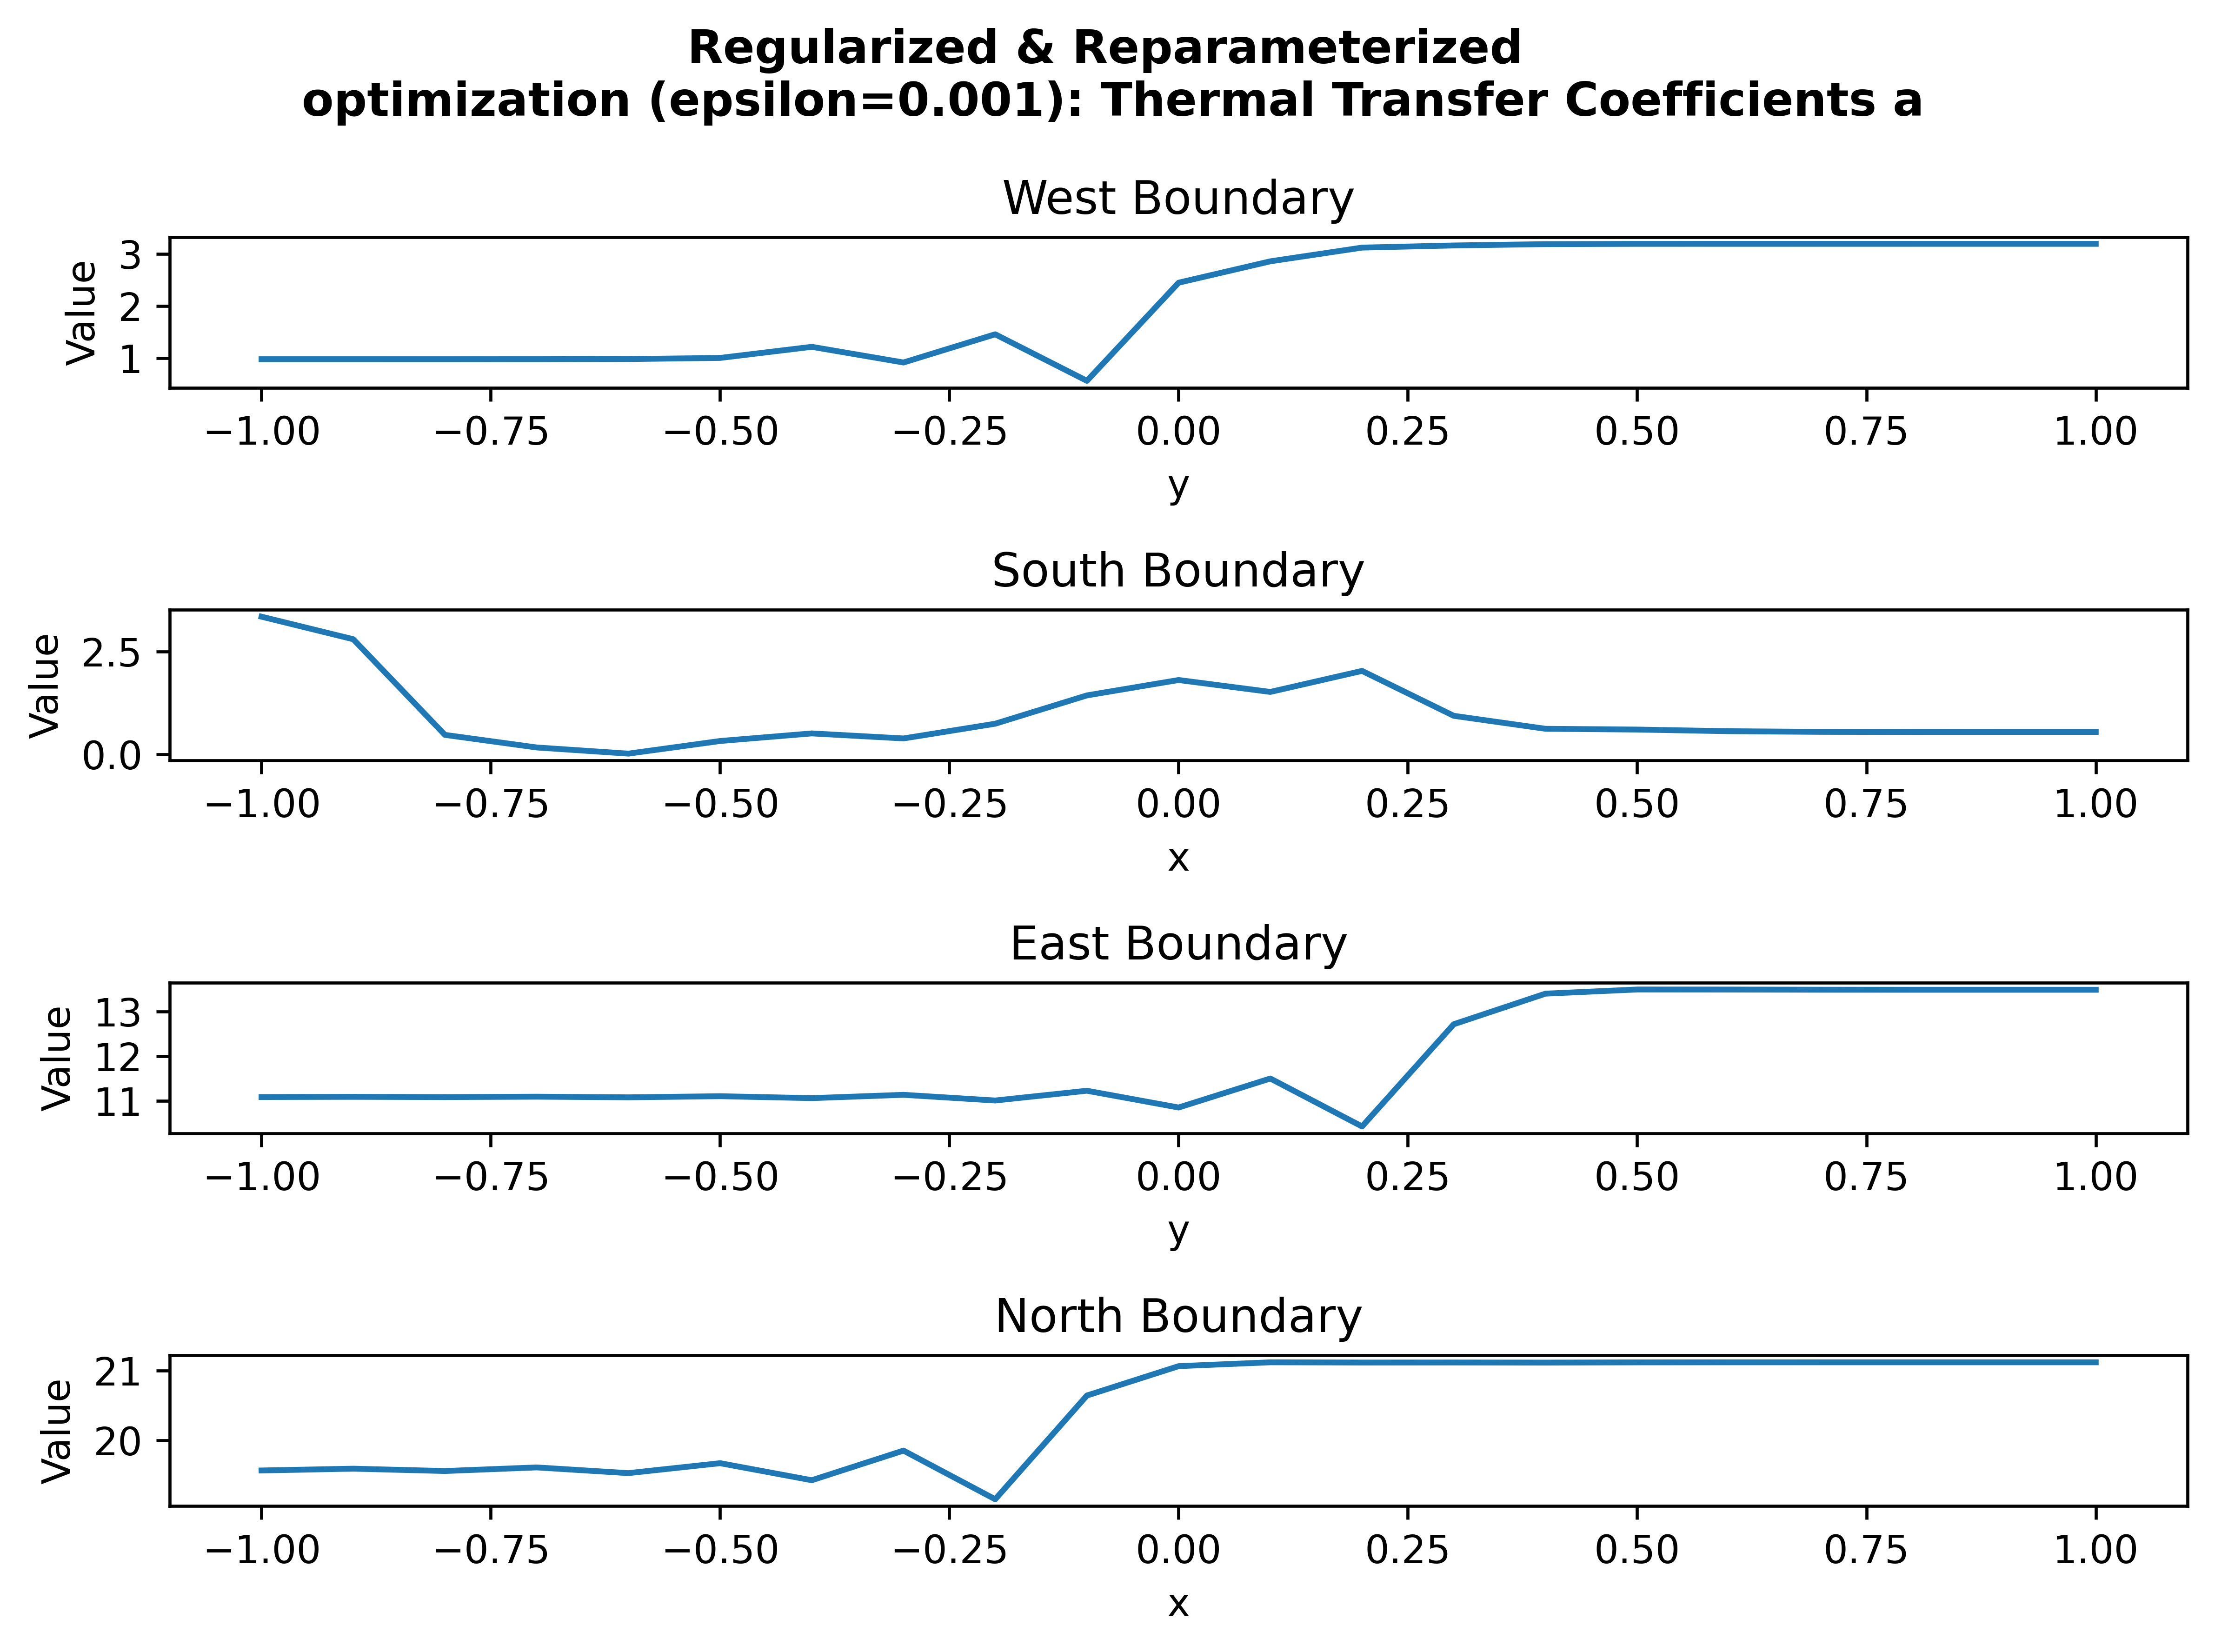
\includegraphics[width=\textwidth]{Project/Part1/Figures/regularized_optimization_epsilon_0.001_a.png}
        \caption{Optimized $a$ solution.}
    \end{subfigure}
    \hfill
    \begin{subfigure}[b]{0.40\textwidth}
        \centering
        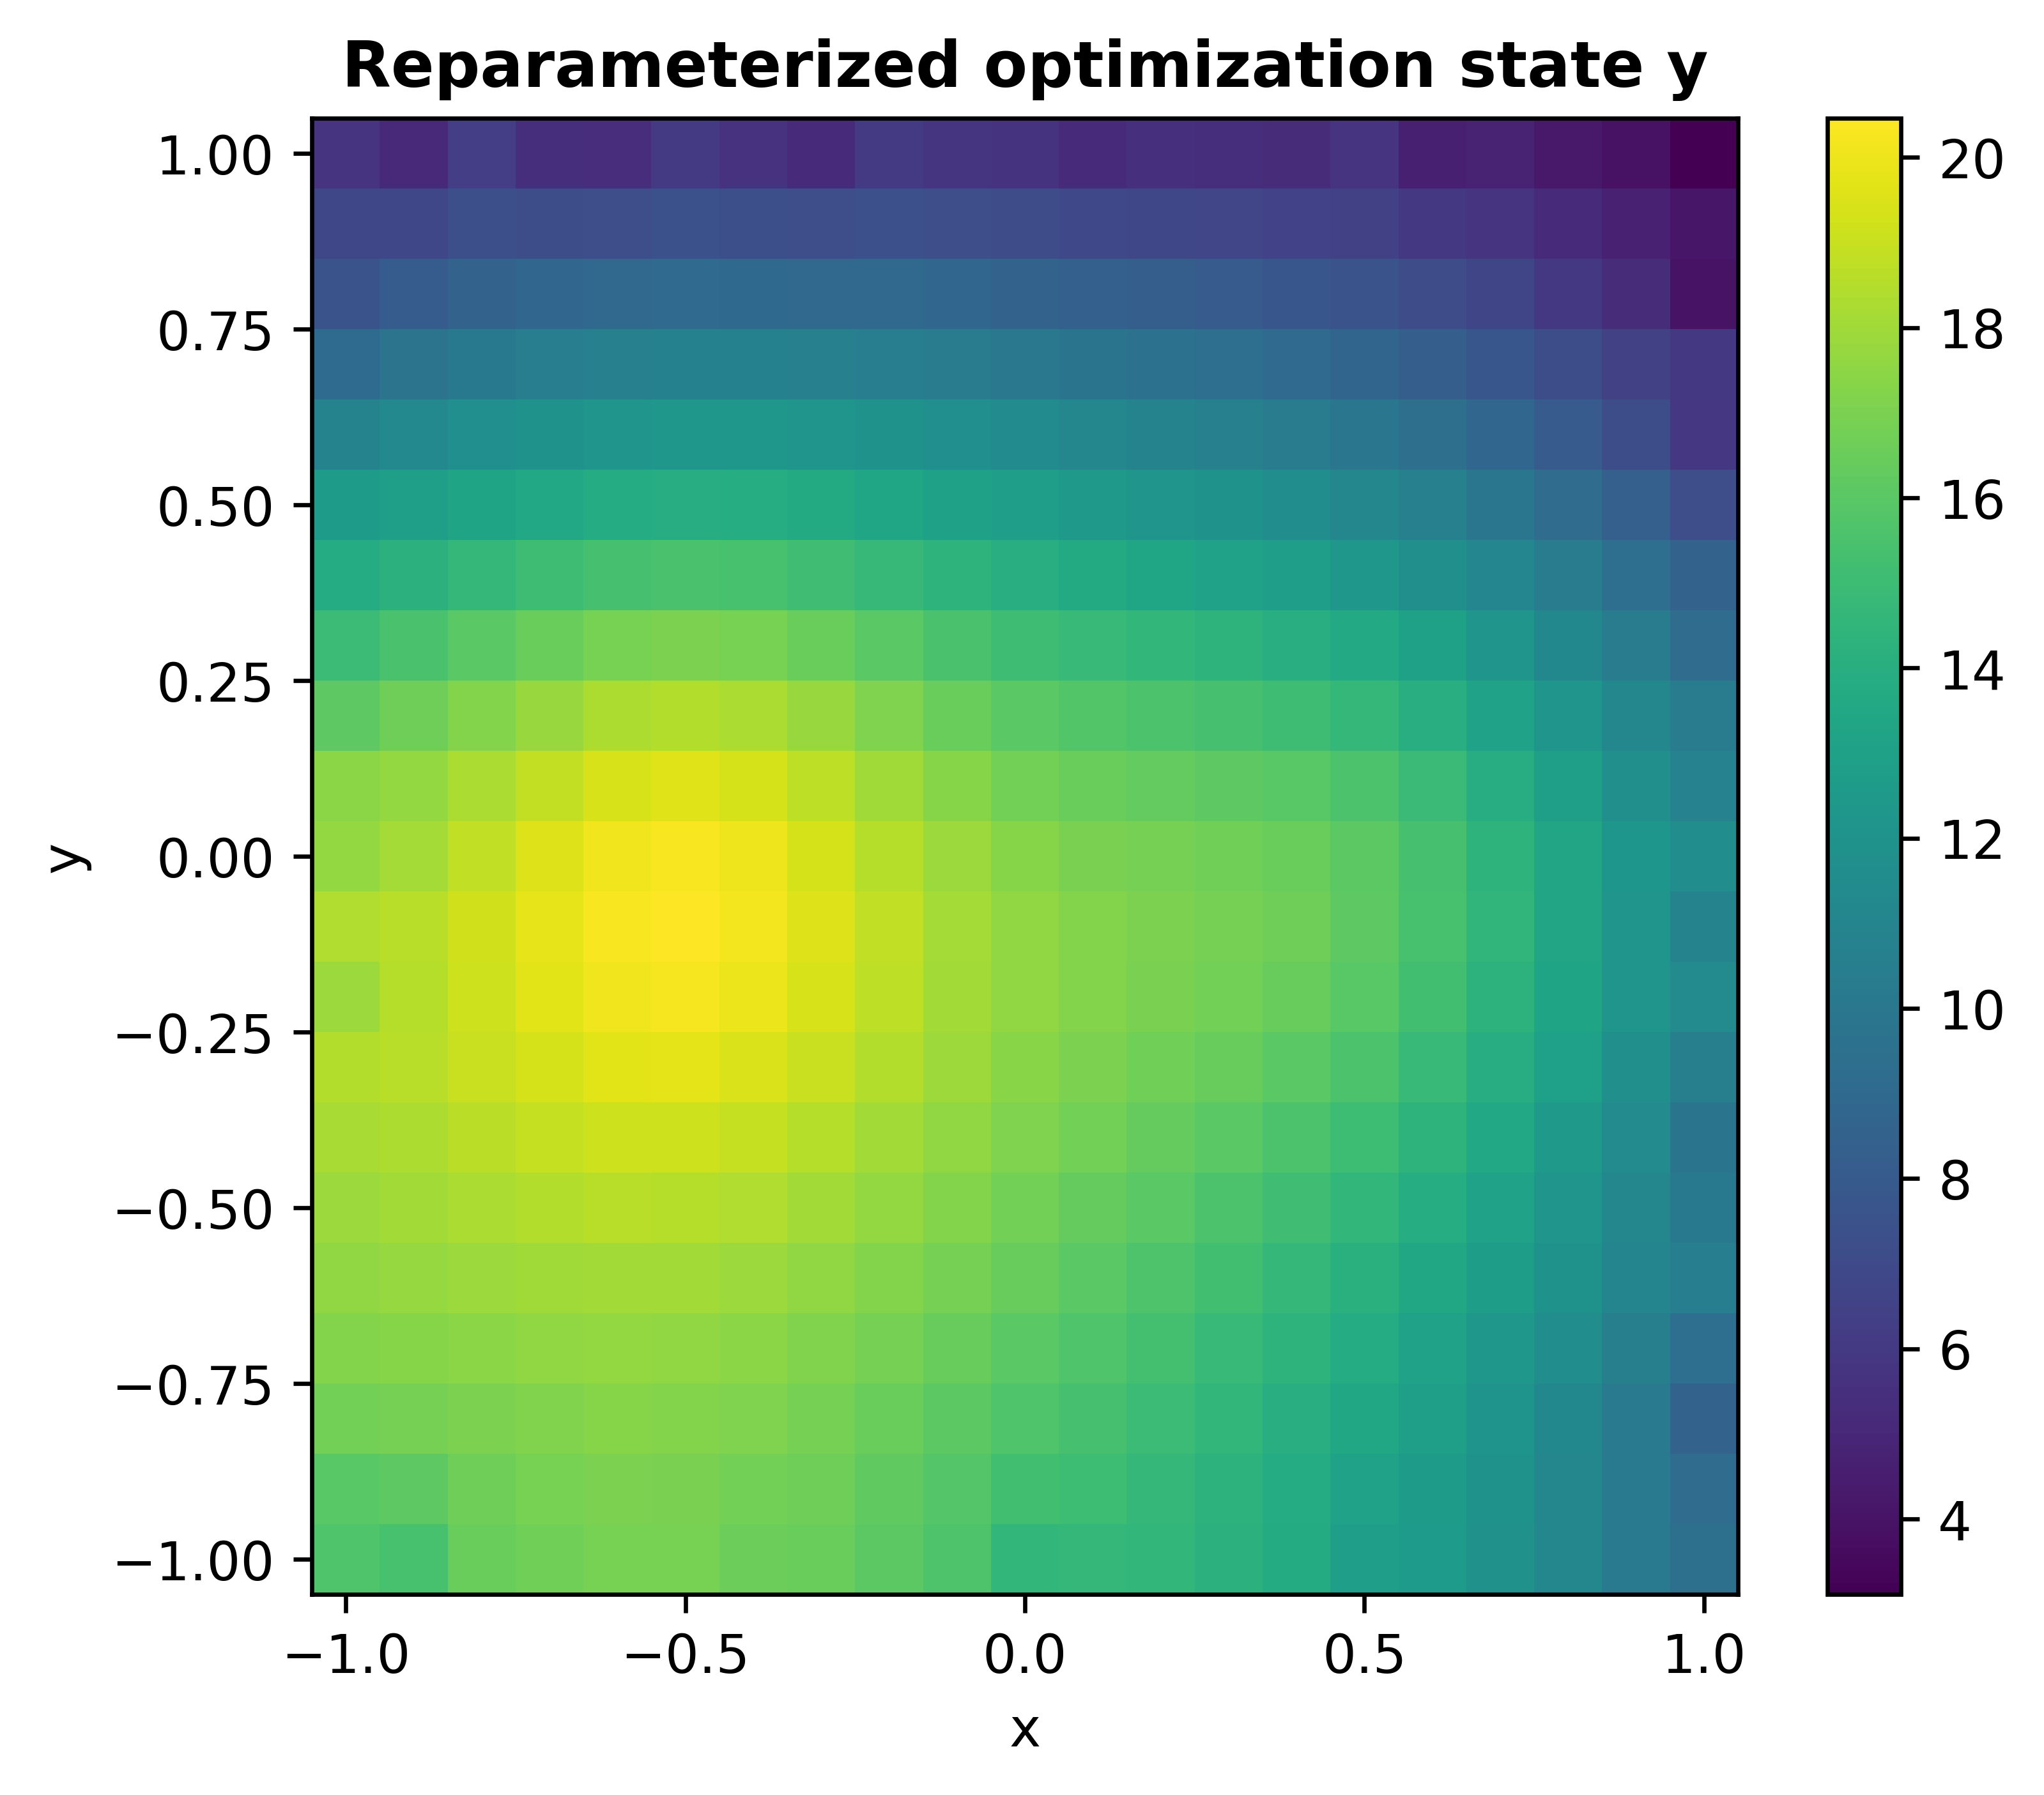
\includegraphics[width=\textwidth]{Project/Part1/Figures/reparam_optimization_y.png}
        \caption{Optimized state $y$.}
    \end{subfigure}
    \caption{Regularized and reparameterized solution of inversion problem ($\varepsilon=10^{-3}$).}
    \label{fig:p1_regularized_optimization}
\end{figure}

\section{Discussion}